\newpage
\chapter{Applicazione del Threat Modeling all'Architettura Proposta}

% \section{Applicazione del Threat Modeling: Modellazione del Sistema}


% Giunti a questo punto, dopo aver analizzato i passi da seguire per modellizzare le minacce possiamo iniziare con il definire il Data Flow Diagram del nostro sistema Smart Grid.

% \begin{figure}[!h]
%     \centering
%     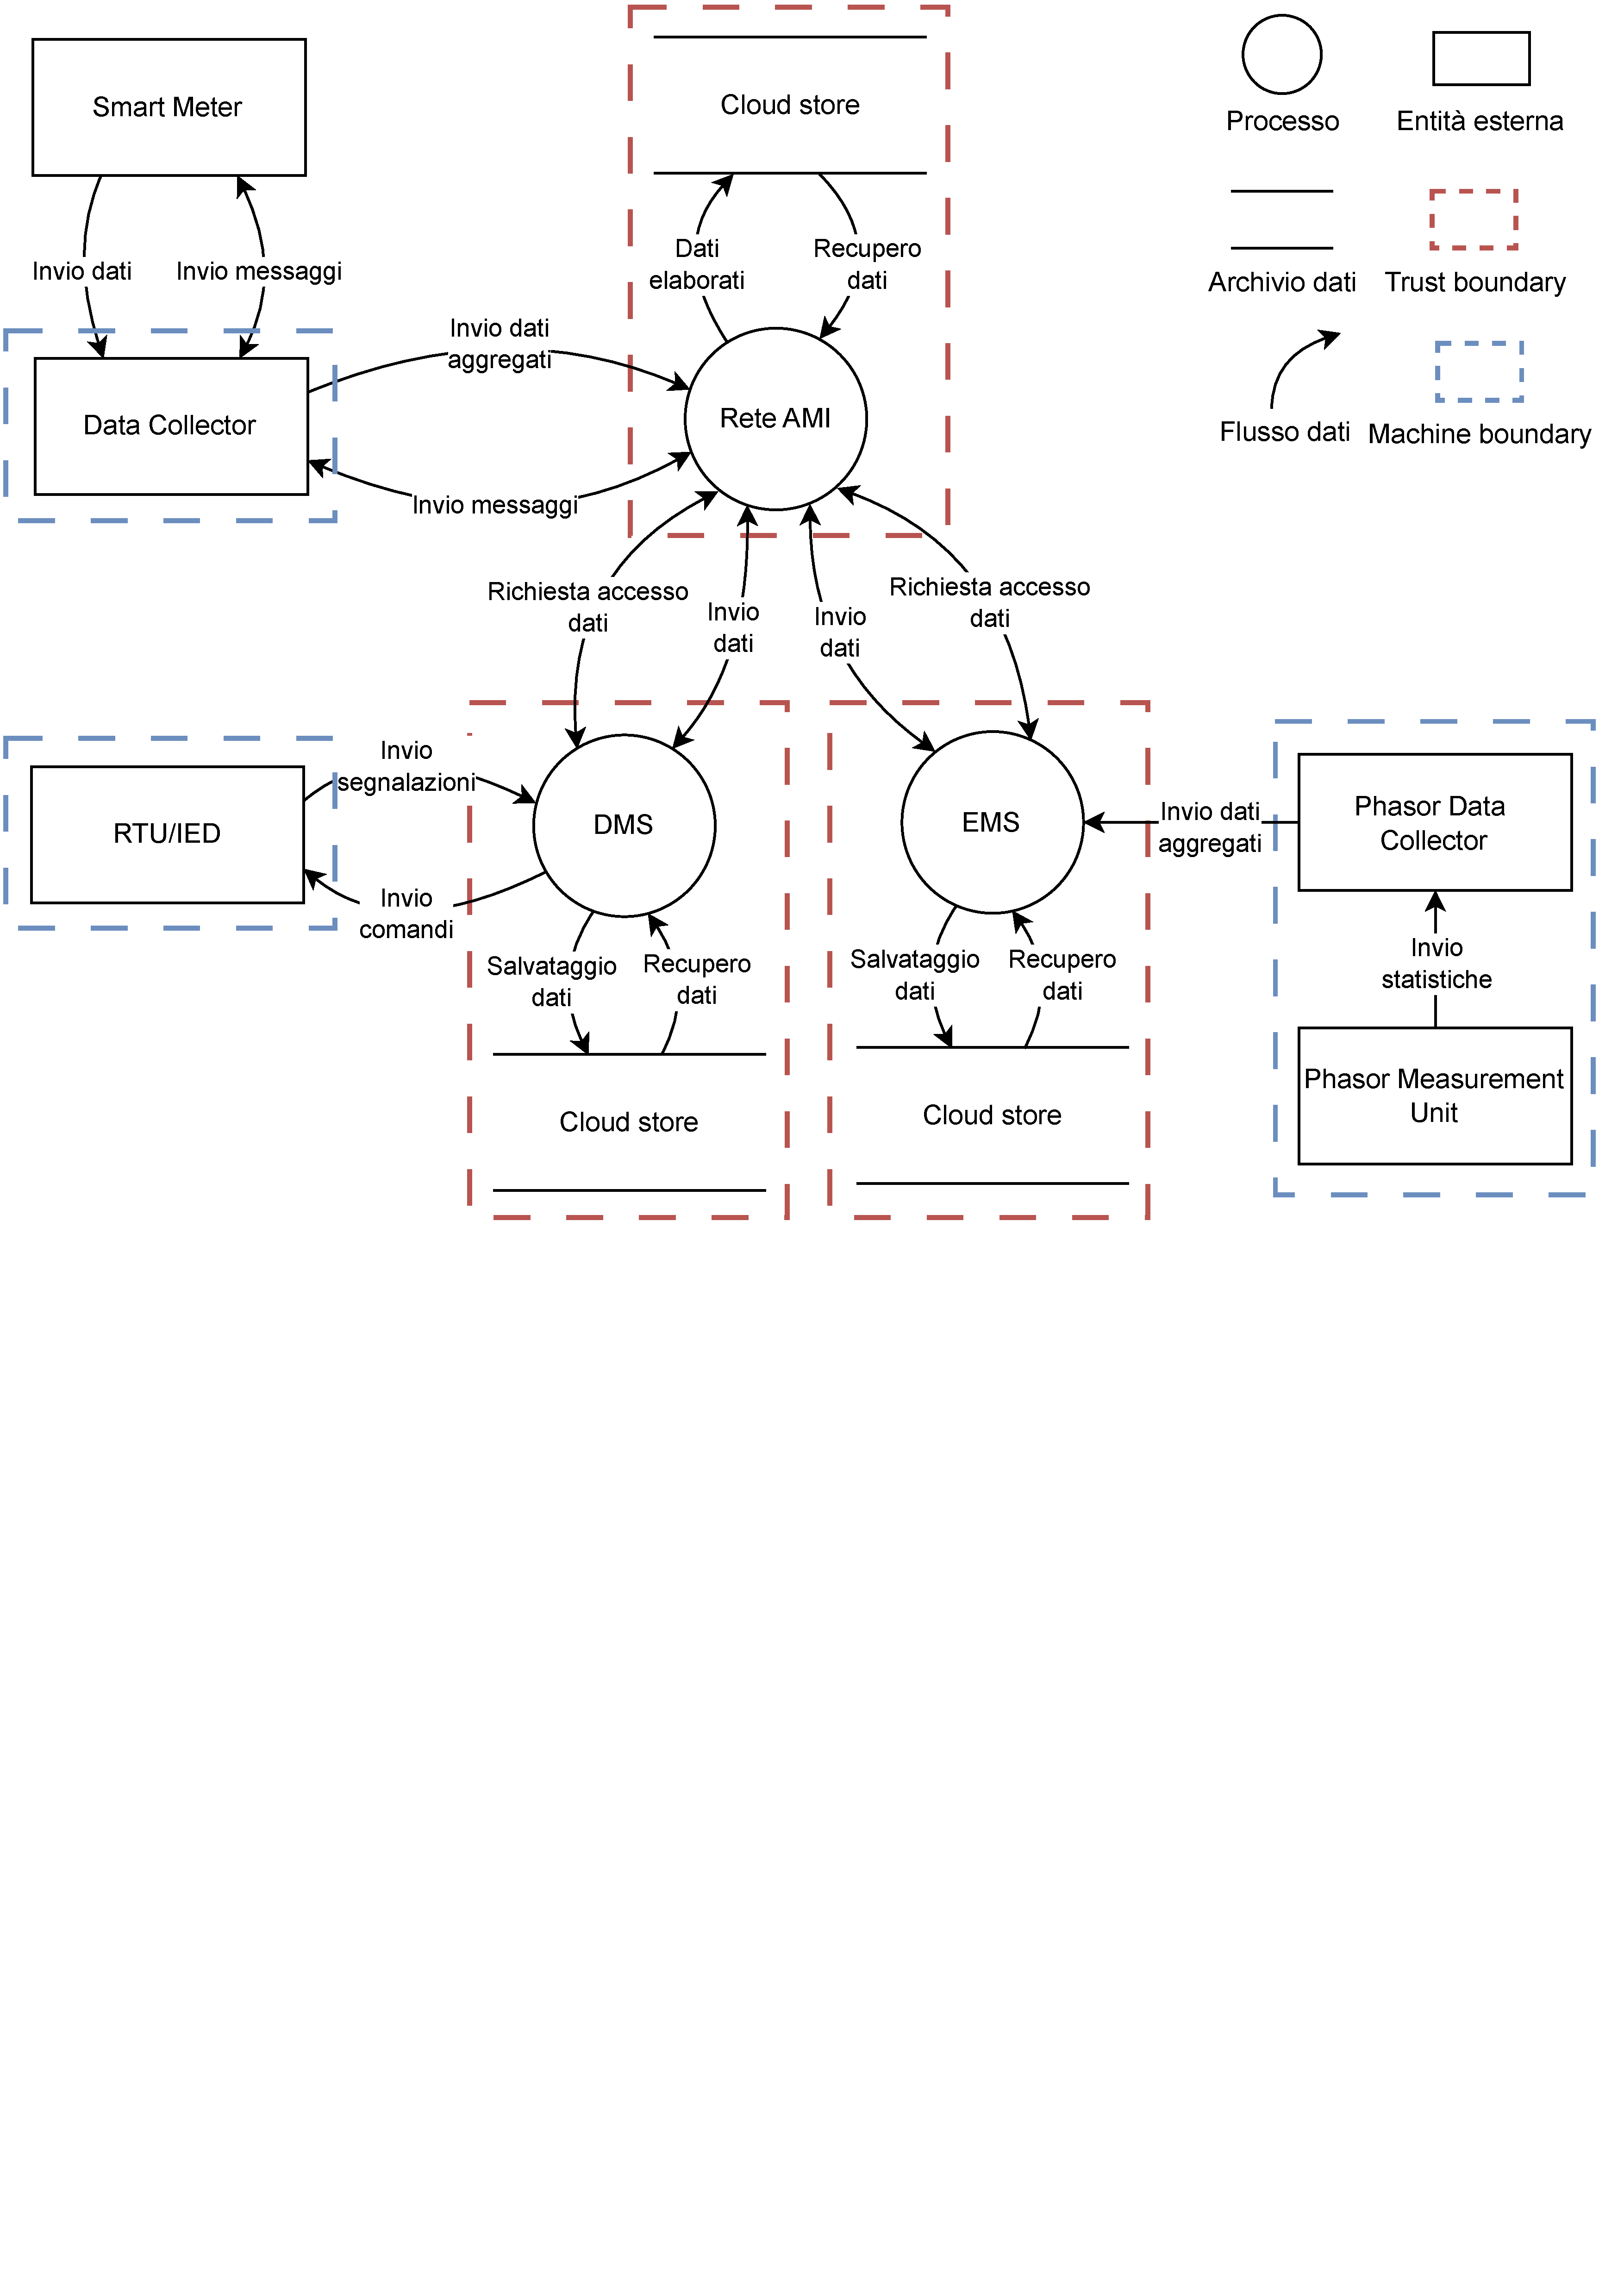
\includegraphics[trim= 0cm 39cm 0cm 0cm, clip, width=0.8\linewidth]{img/DFD.drawio.pdf}
%     \caption{Data flow diagram - Smart Grid Cloud-Native}
%     \label{fig:DFD}
% \end{figure}

% Come si vede dalla Figura \ref{fig:DFD}, visione semplificata delle componenti cardine, sono stati identificati dei \textit{Boundaries}, ovvero dei confini sicuri, che possono essere di due tipologie:

% \begin{itemize}

%     \item Trust Boundaries (rossi): generici confini di sicurezza, garantiti di fatto dalla presenta dell'architettura Cloud-Native.
%     \item Machine Boundaries (blu): questi sono dei confini di sicurezza fisici, che proteggono i componenti sul campo da possibili manomissioni.
% \end{itemize}

Nei capitoli precedenti sono stati definiti i tre pilastri concettuali di questa tesi: il concetto di Smart Grid con la sua architettura e componenti (Capitolo 1), un'implementazione di una Smart Grid basata su un paradigma \textit{Cloud-Native} (Capitolo 2) e la metodologia formale del \textit{Threat Modeling} per l'analisi della sicurezza dei sistemi (Capitolo 3).

Questo capitolo rappresenta il punto di convergenza di questi tre elementi, costituendo il contributo centrale della ricerca. L'obiettivo è applicare sistematicamente il processo di \textit{Threat Modeling}, e in particolare il framework STRIDE, al modello architetturale proposto, al fine di identificare e classificare le principali minacce informatiche che lo caratterizzano.


L'analisi seguirà fedelmente le quattro fasi metodologiche descritte in precedenza:

\begin{enumerate}
    \item \textbf{Modellazione del Sistema:} Verrà presentato e discusso in dettaglio il \textit{Data Flow Diagram} (DFD) dell'architettura.
    \item \textbf{Identificazione delle Minacce:} Ogni componente del DFD verrà analizzato attraverso la lente di STRIDE per enumerare le potenziali minacce.
    \item \textbf{Mitigazione delle Minacce:} Per le minacce più significative, verranno proposte delle contromisure di sicurezza specifiche per il contesto \textit{Cloud-Native}.
    \item \textbf{Validazione:} Verrà discusso un piano di validazione delle minacce.
\end{enumerate}


% \section{Modellazione del Sistema}
\section{Definizione del Data Flow Diagram}

In questa sezione si avvia l'applicazione pratica del processo di \textit{Threat Modeling} all'architettura Smart Grid \textit{Cloud-Native} proposta. Il primo passo fondamentale, come descritto dalla metodologia, consiste nella modellazione del sistema attraverso un DFD.

La  Figura \ref{fig:DFD} presenta un DFD di Livello 0 che astrae l'architettura, evidenziandone i componenti principali, i flussi di dati e, soprattutto, i confini di sicurezza. In questo modello sono stati identificati i seguenti elementi:

\begin{itemize}
    \item \textbf{Entità Esterne:} Componenti che interagiscono con il sistema ma si trovano al di fuori del suo controllo diretto, come lo \textit{Smart Meter}, l'RTU/IED e il sistema PMU/PDC.
    \item \textbf{Processi:} I componenti software che elaborano i dati, come l'AMI, il DMS e l'EMS.
    \item \textbf{Archivi Dati:} I luoghi di memorizzazione dei dati, rappresentati dai \textit{Cloud Store}.
\end{itemize}

Per l'analisi di sicurezza, sono stati definiti due tipi di confini (\textit{boundaries}), ciascuno con un significato preciso:

\begin{enumerate}
    \item \textbf{\textit{Trust Boundary} (confine rosso):} Rappresenta un confine logico che separa componenti con diversi livelli di fiducia. Qualsiasi flusso di dati che attraversa un \textit{Trust Boundary} deve essere considerato potenzialmente ostile e quindi soggetto a rigorose procedure di autenticazione, autorizzazione e validazione. Questi confini definiscono la superficie di attacco di ciascun servizio.
    \item \textbf{\textit{Machine Boundary} (confine blu):} Rappresenta un confine fisico o a livello di dispositivo. Esso isola i componenti che operano sul campo (\textit{Edge}), come il \textit{Data Concentrator} o il \textit{Phasor Data Concentrator}, dal loro ambiente fisico e dalla rete locale. Questo confine è rilevante per analizzare minacce di accesso fisico (manomissione) o attacchi diretti al dispositivo, che bypasserebbero i controlli a livello di applicazione.
\end{enumerate}

% Questo DFD, con la sua chiara distinzione tra processi, dati e confini, costituisce la mappa fondamentale su cui, nella fase successiva, verranno sistematicamente identificate le minacce utilizzando il framework STRIDE.



\begin{figure}[!h]
    \centering
    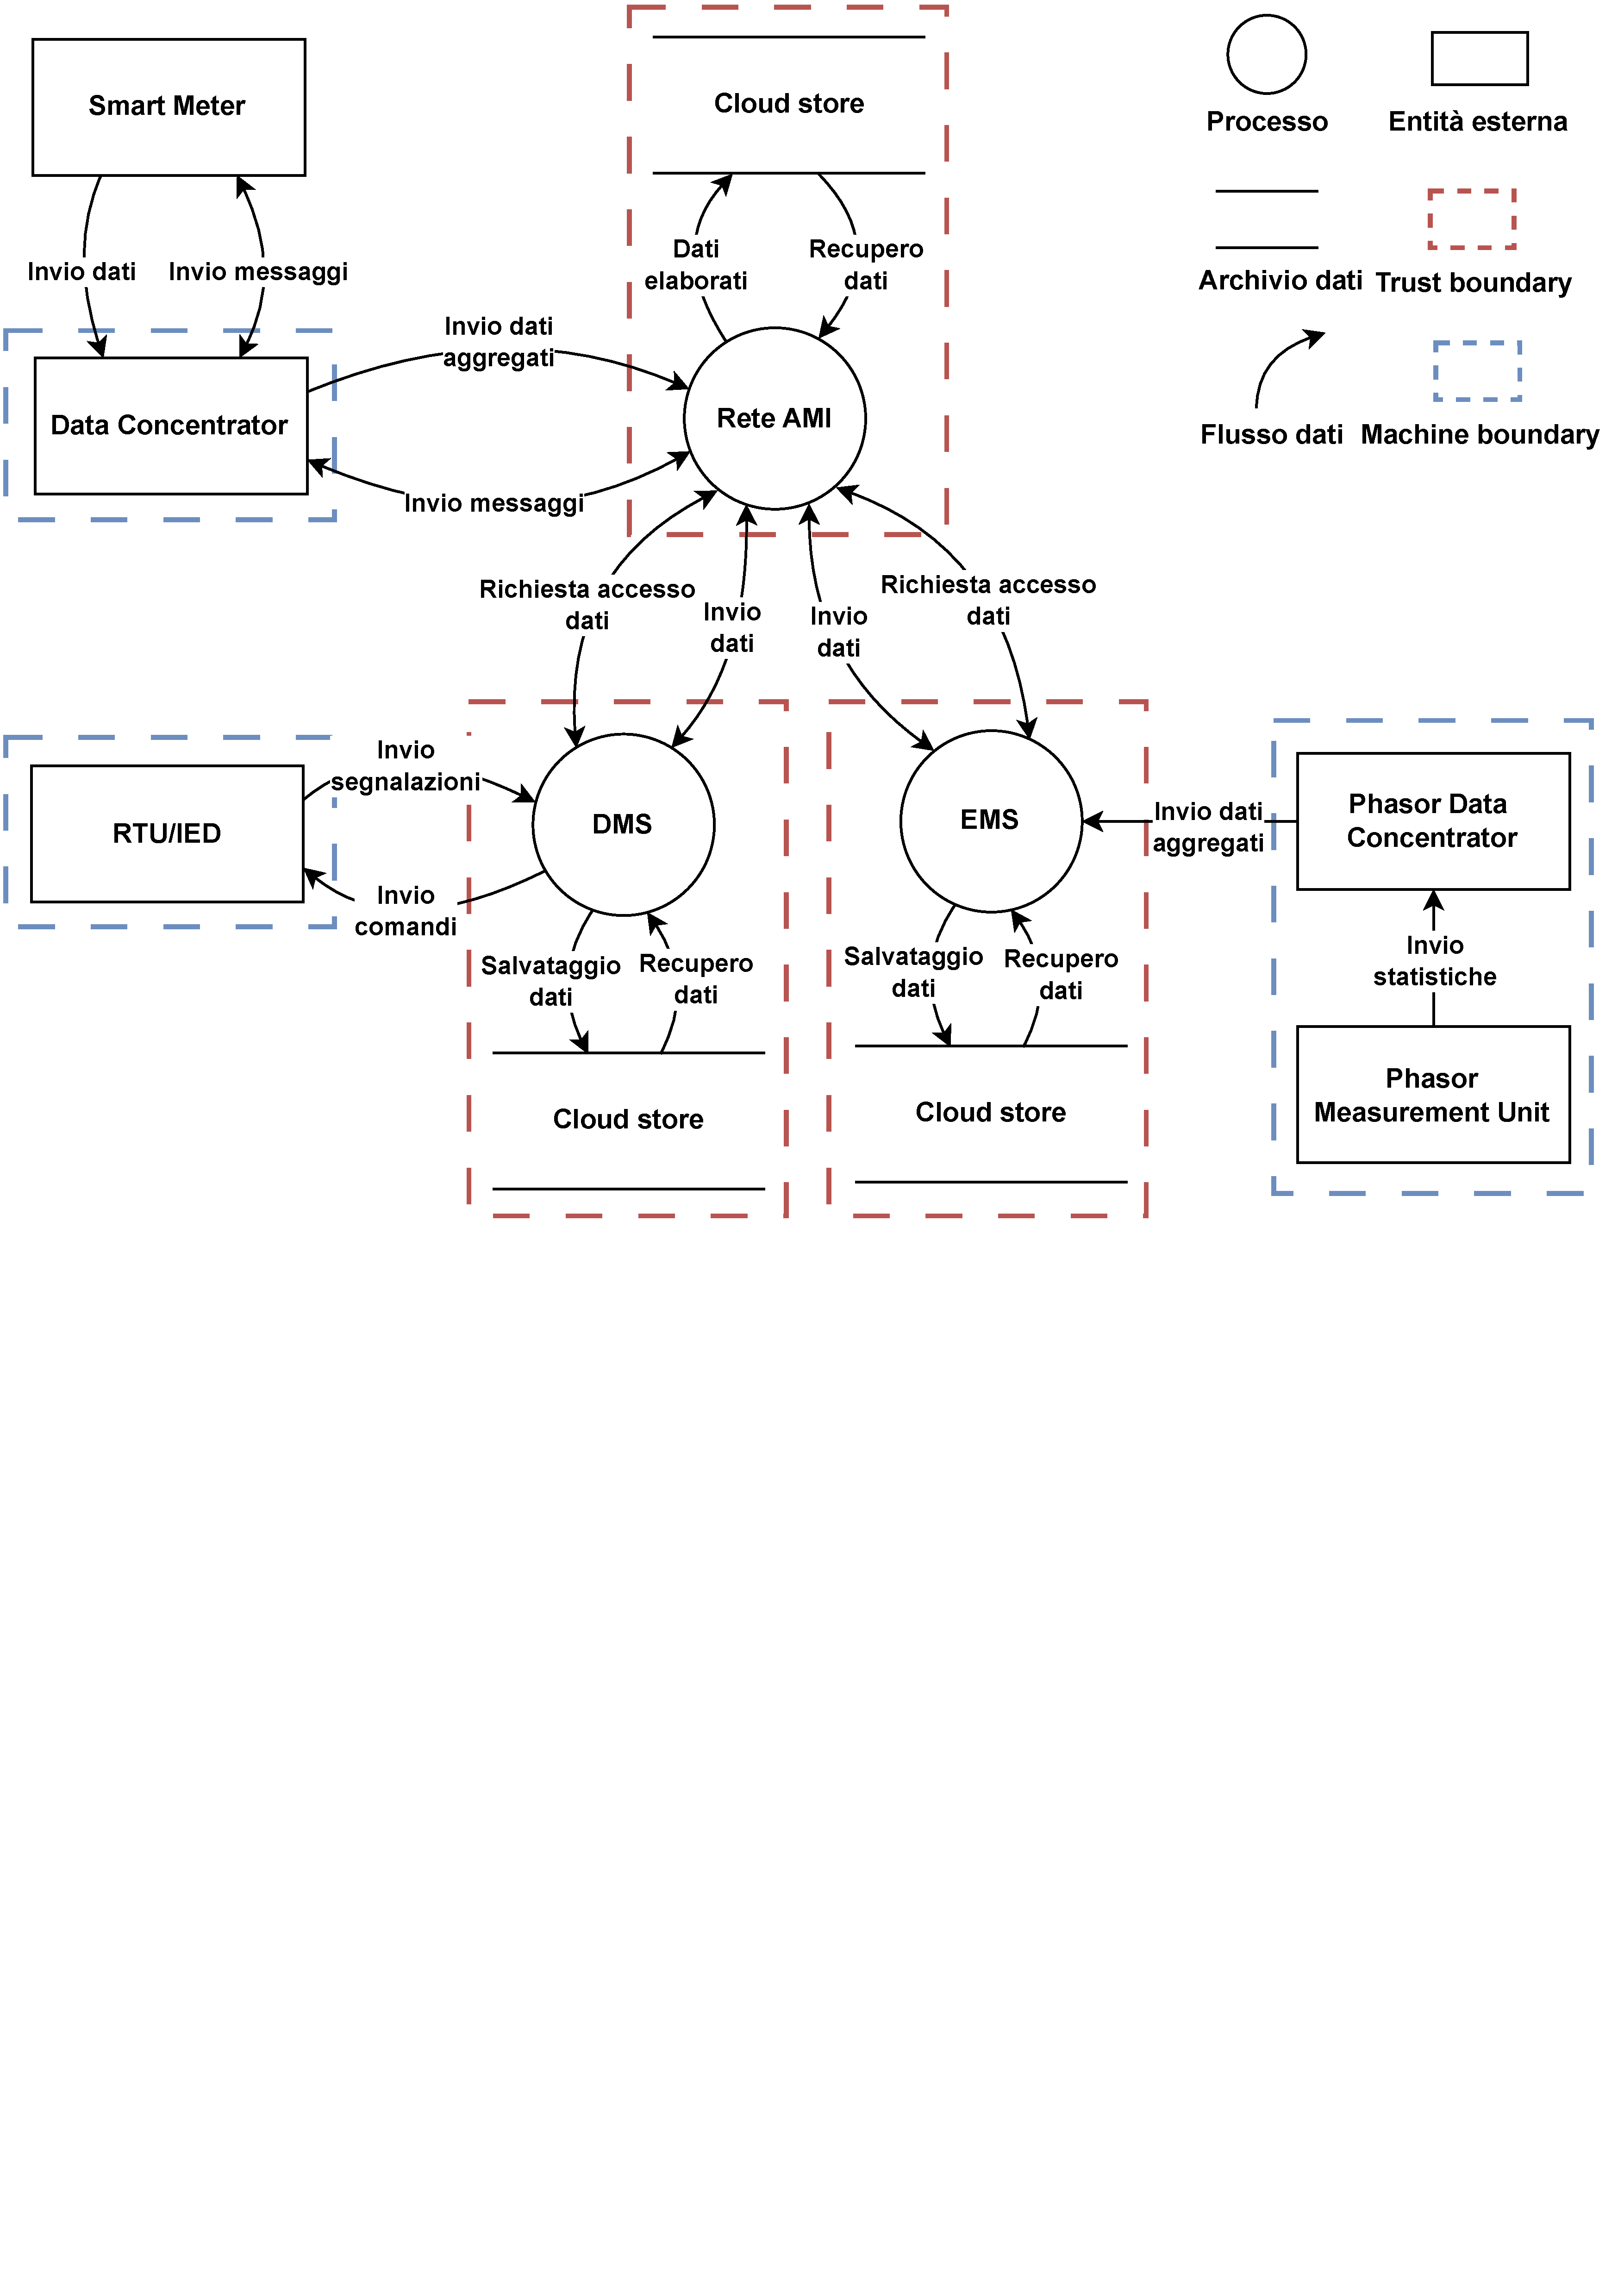
\includegraphics[trim= 0cm 39cm 0cm 0cm, clip, width=0.8\linewidth]{img/DFD.drawio-v2.drawio.pdf}
    \caption{Data flow diagram - Smart Grid Cloud-Native}
    \label{fig:DFD}
\end{figure}


\subsection{Definizione dell'Ambito di Analisi}

% Nella Tabella \ref{tab:def-ambito} troviamo la definizione degli elementi: \textit{In scope}, ovvero all'interno dell'ambito di ricerca di questa tesi; \textit{Out od scope}, che non fanno parte prettamente all'infrastruttura cloud della Smart Grid. 

Prima di procedere con l'analisi delle minacce, è essenziale definire con precisione il perimetro (\textit{scope}) di questo studio. Data la vastità dell'ecosistema Smart Grid, l'analisi si concentrerà specificamente sulle vulnerabilità introdotte dalla sua implementazione in un'architettura \textit{Cloud-Native}.


Di conseguenza, verranno prese in considerazione le minacce relative ai componenti software centralizzati e ai canali di comunicazione che li collegano al campo. 
% Le problematiche di sicurezza legate strettamente all'hardware dei dispositivi Edge – come la manomissione fisica, gli attacchi a livello di firmware o le vulnerabilità dei circuiti integrati – pur essendo di fondamentale importanza per la sicurezza complessiva, sono considerate al di fuori dell'ambito di questa tesi per mantenere un focus mirato sulle minacce a livello di architettura di rete e applicativa.


La Tabella \ref{tab:def-ambito} riassume formalmente questa suddivisione, elencando gli elementi considerati oggetto di analisi (\textit{In Scope}) e esclusi dall'analisi (\textit{Out of Scope}).

% \begin{table}[h!]
%     \centering
%     % \renewcommand{\arraystretch}{1.5}
    
%     \begin{tabular}{c|c|c}
%          &  \textbf{In scope} & \textbf{Out of scope}\\
%          \hline
%          &  & \\
%          Componenti  &   HES, MDMS, DMS, EMS, & Sicurezza dei dispositivi hardware: SM, DC, \\         
%          software: &   SCADA, GMS, High-level PDC & RTU/IED, Generatori, low-level PDC, PMU\\
%         &  & \\
         
%          Canali di &  PLC/RF $169\,MHz$, 4G/5G,&  Sicurezza della cabina Telco\\
%          comunicaizone: &    Fibra, VPN  & \\
%           &  & \\
%          Infrastruttura cloud:&  Kubernetes e container & \\
%           &  & \\
%     \end{tabular}
%     \caption{Definizione dell'ambito}
%     \label{tab:def-ambito}
% \end{table}

\renewcommand{\arraystretch}{1.5}
\begin{longtable}[!h]{p{5cm}p{5cm}p{5cm}}
        
    \caption{Definizione dell'ambito di analisi} 
    \label{tab:def-ambito}\\
    
    \hline
    &  \textbf{Oggetto in analisi} & \textbf{Oggetto fuori dall'analisi}\\
    \hline
    \endfirsthead
    
    \hline
    &  \textbf{Oggetto in analisi} & \textbf{Oggetto fuori dall'analisi}\\
    \hline
    \endhead

    Componenti software: &   SM, HES, MDMS, DMS, EMS, SCADA, GMS, High-level PDC & Sicurezza dei dispositivi hardware: DC, RTU/IED, Generatori, low-level PDC, PMU\\
    
    Canali di comunicazione: &  PLC/RF $169\,MHz$, 4G/5G, Fibra, VPN&  Sicurezza della cabina Telco\\
         
    Infrastruttura cloud:&  Kubernetes e container & \\

    
    \hline
\end{longtable}

\newpage
\subsection{Identificazione degli Asset Critici}

% Nella seguente Tabella \ref{tab:def-asset}, in ogni colonna, sono presentati una serie di asset


% \begin{table}[h!]
%     \centering
%     \renewcommand{\arraystretch}{1.5}
    
%     \begin{tabular}{c|c|c}
%          \textbf{Dati} &  \textbf{Processi} & \textbf{Infrastruttura logica}\\
%          \hline
%          Statistiche del cliente   &    dati collezionati da HES & Cluster K8s  \\         
%          Fatturazione consumi (MDMS) &   elaborazione dei dati MDMS & Immagini container \\
%          Statistiche di rete (PMU) &  monitoraggio della rete EMS/DMS & Infrastruttura VPN \\
         
%          API, credenziali, token & Dati collezionati da high-level PDC & Cloud storage  \\

%     \end{tabular}
%     \caption{Definizione degli asset}
%     \label{tab:def-asset}
% \end{table}



Successivamente alla definizione della struttura del sistema tramite il DFD, è cruciale identificare gli asset, ovvero gli elementi di valore all'interno dell'architettura la cui compromissione causerebbe un danno significativo. Sapere cosa si sta proteggendo è un prerequisito fondamentale per poter valutare l'impatto reale di una minaccia.
Un'analisi completa considera che gli asset non sono limitati ai soli dati, ma includono anche i processi e i componenti infrastrutturali che li gestiscono. Per questa tesi, gli asset sono stati classificati in tre tipologie principali:

\begin{enumerate}
    \item \textbf{Dati:} Rappresentano le informazioni sensibili o critiche gestite dal sistema. La loro compromissione può portare a violazioni della privacy, frodi o perdita di controllo sulla rete. Esempi includono i dati di consumo dei clienti, le statistiche di rete delle PMU e le credenziali di accesso come token e chiavi API.
    \item \textbf{Processi:} Sono le funzioni operative e di elaborazione chiave del sistema. Un attacco a un processo può corrompere i dati, causare un'interruzione del servizio o portare a decisioni errate nella gestione della rete. Esempi includono l'elaborazione dei dati da parte dell'MDMS o il monitoraggio della rete da parte dell'EMS.
    \item \textbf{Infrastruttura Logica:} Costituisce la base tecnologica su cui poggia l'intera architettura. La compromissione di questi componenti può avere un impatto a cascata su tutti i servizi ospitati. Esempi includono i cluster Kubernetes, le immagini dei container e l'infrastruttura VPN che garantisce la comunicazione sicura.
\end{enumerate}

La Tabella \ref{tab:def-asset} presenta una sintesi dei principali asset identificati per l'architettura in esame, classificati secondo queste tre tipologie.

\renewcommand{\arraystretch}{1.5}
\begin{longtable}[!h]{p{5cm}p{5cm}p{5cm}}
        
    \caption{Identificazione degli Asset Critici}
    \label{tab:def-asset}\\
    
    \hline
    \textbf{Dati} &  \textbf{Processi} & \textbf{Infrastruttura logica}\\
    \hline
    \endfirsthead
    
    \hline
    \textbf{Dati} &  \textbf{Processi} & \textbf{Infrastruttura logica}\\
    \hline
    \endhead
    
    
    Statistiche del cliente   &    Dati collezionati da HES & Cluster K8s  \\         
    Fatturazione consumi (MDMS) &   Elaborazione dei dati MDMS & Immagini container \\
    Statistiche di rete (PMU) &  Mnitoraggio della rete EMS/DMS & Infrastruttura VPN \\    
    API, credenziali, token & Dati collezionati da high-level PDC & Cloud storage  \\
    
    
    \hline
\end{longtable}

\newpage
\section{Analisi delle Minacce con il Framework STRIDE}

Dopo aver modellato il sistema, si procede ora con la fase di identificazione delle minacce, il cuore di questa analisi. Come anticipato, questa fase verrà condotta applicando sistematicamente il framework STRIDE e utilizzando come riferimento il \textit{Data Flow Diagram} Figura \ref{fig:DFD}.


L'approccio utilizzato sarà quello di STRIDE-per-elemento: per ogni componente del DFD (processi, \textit{data store}, flussi di dati ed entità esterne), verranno considerate le categorie di minaccia STRIDE pertinenti. Questo metodo garantisce una copertura completa e strutturata, riducendo il rischio di tralasciare vulnerabilità significative.




% \renewcommand{\arraystretch}{1.5}
% \begin{longtable}{p{1.5cm}p{2cm}p{2cm}p{6.5cm}p{3cm}}
%     \caption{Minacce informatiche}
%     \label{tab:minacce-info} \\
    
%     \hline
%     \textbf{ID Minaccia} &\textbf{Elemento} & \textbf{Categoria STRIDE}& \textbf{Descrizione minaccia} & \textbf{Possibile attaccante} \\
%     \hline
%     \endfirsthead
    
%     \hline
%     \textbf{ID Minaccia} &\textbf{Elemento} & \textbf{Categoria STRIDE} & \textbf{Descrizione minaccia} &\textbf{Possibile attaccante} \\
%     \hline
%     \endhead

%     S-01 & Cluster K8s & \textbf{S}poofing, Elevation of Privilege & Service Account Impersonation: un attaccante sfrutta una vulnerabilità di un pod per impossessarsi della private key del suo Service Account e lo usa per accedere alle API di K8s, impersonando il servizio per leggere configurazione e lanciare altri pod malevoli. & Attaccante esterno che ha ottenuto un accesso iniziale; insider\\
    
%     T-01 & Nodi worker K8s &  \textbf{T}ampering, Elevation of Privilege & Un attaccante sfruttando una vulnerabilità del cloud provider, modifica in una qualsiasi parte il worker node di K8s permettendogli di inserire del codice malevole per prenderne il possesso. & Attaccante molto competente\\

%     T-02 & Comunicazioni & \textbf{T}ampering & Un attaccante riesce ad intercettare la comunicazione, da e/o verso un servizio cloud, modificandone i dati di consumo o comandi di esecuzione. Man-in-the-middle attack. & Attaccante esterno con accesso alla rete di comunicazione (PLC, VPN, Fibra)\\

%     R-01 & Invio comandi & \textbf{R}epudiation & Un operatore di un sistema (EMS/DMS) invia un comando alla rete, di trasformazione, produzione, ecc., legittimo ma dannoso per errore e poi nega di averlo fatto. La mancanza di log immutabili e firmati digitalmente rende impossibile l'attribuzione del fatto. & Operatore interno \\
    

%     I-01 & Flussi dati & \textbf{I}nformation Disclosure & A causa di regole di firewall assenti o troppo permissive tra i cluster K8s, un attaccante può sfruttare le porte lasciate aperte per sferrare l'attacco & Attaccante esterno \\

%     I-02 & Comunicazione in entrata & \textbf{I}nformation Disclosure & Le regole impostate del firewall risultano essere troppo permissive, esponendo su internet i nodi dei cluster, incluse porte sensibili come la porta 22 (SSH) la quale può essere presa di mira dagli attaccanti. & Attaccante esterno \\

%     I-03 & Dati salvati & \textbf{I}nformation Disclosure & Un utente interno o un possibile attaccante sfruttando configurazioni errate del cloud storage per accedere ai dati dei clienti o allo stato della rete. & Insider; Attaccante esterno\\

%     D-01 & Disponibilità servizio & \textbf{D}enial of Service & Un attaccante lancia un attacco DDoS contro gli endpoint della della rete, impedendo agli operatori l'analisi della rete in tempo reale & Attaccante esterno \\

%     E-01 & Cluster K8s & \textbf{E}levation of Privilege &  Non rispetto del principio del minimo privilegio, assegnando al personale ruoli di accesso non pertinenti alla sua mansione & Insider\\

%     E-02 & \textbf{E}levation of Privilege & Processi interni al cluster K8s & Un attaccante, dopo aver compremesso un pod con bassi privilegi, sfrutta una vulnerabilità del container runtime o del kernel per ottenere l'accesso root sul nodo, potendo così inviare messaggi malevoli alla rete & Attaccante esterno \\
   

% \hline

% \end{longtable}

\renewcommand{\arraystretch}{1.5}
\begin{longtable}{p{1.5cm}p{2cm}p{2cm}p{7.5cm}p{2cm}}
    \caption{Minacce informatiche}
    \label{tab:minacce-info} \\
    
    \hline
    \textbf{ID Minaccia} &\textbf{Elemento} & \textbf{Categoria STRIDE}& \textbf{Descrizione minaccia} & \textbf{Possibile attaccante} \\
    \hline
    \endfirsthead
    
    \hline
    \textbf{ID Minaccia} &\textbf{Elemento} & \textbf{Categoria STRIDE} & \textbf{Descrizione minaccia} &\textbf{Possibile attaccante} \\
    \hline
    \endhead

    S-01 & Smart Meter & \textbf{S}poofing & Una mancanza di risorse e memoria limitata su SM e dispositivi di campo, possono impedire l'implementazione di tutte le funzionalità di sicurezza e l'aggiornamento del firmware, rendendoli più vulnerabili ad attaccanti esperti che riescono a sfruttare queste vulnerabilità minando l'affidabilità dei dati inviati ai DC. \cite{paper-threat-modelling}& Attaccante esterno\\
    
    T-01 & Flusso dati PDC & \textbf{T}ampering & Un attaccante non si limita ad un possibile DoS bloccando i dati inviati dai PDC su rete 4G/5G, bensì cerca di intercettare il traffico e modificare leggermente e costantemente tutti i dati prima che essi raggiungano l'EMS. Questo attacco simula un carico fantasma o una falsa instabilità di frequenza. L'EMS che si fida di questi dati reagisce automaticamente ridirigendo l'energia o sezionando la zona, causando gravi disagi. \cite{paper-threat-modelling}& Attaccante esterno\\

    R-01 & Dati consumatori & \textbf{R}epudiation & Un attaccante esterno, riuscendo ad avere accesso privilegiato con permessi di lettura e scrittura al \textit{cloud store} dell'infrastruttura AMI, riesce a modificare i dati contenuti nel database con conseguente impatto sulle misure fino ad ora effettuate e possibili previsioni future. & Attaccante esterno \\
    

    I-01 & Software di gestione & \textbf{I}nformation Disclosure & Un attaccante può sfruttare le vulnerabilità scoperte nei software \textit{open source}, come ad esempio OpenEMS, per compromettere i sistemi EMS delle aziende che li utilizzano. Alternativamente, l'attaccante può inserire codice malevolo nel progetto \textit{open source}, che successivamente utilizzerà per condurre attacchi mirati all'esfiltrazione dei dati dell'azienda. & Attaccante esterno\\

    D-01 & Disponibilità servizio & \textbf{D}enial of Service & L'attaccante riesce ad accedere alle cabine secondarie del DSO e si collega tramite uno \textit{switch} tra il \textit{gateway} e la RTU. Questa posizione privilegiata gli consente di intercettare il traffico di rete e identificare il server SCADA presente nel DMS. Una volta individuato il target, l'attaccante può lanciare un attacco DoS (magari utilizzando un software come \textit{hping}) contro il servizio cloud che ospita il cluster Kubernetes, saturando il canale di trasmissione e causando latenze significative (\textit{Bottleneck}). Queste latenze compromettono gravemente l'invio tempestivo dei dati di telemetria, delle segnalazioni e dei comandi di controllo provenienti dallo SCADA Master, causando potenziali disfunzioni operative nella rete di distribuzione. \cite{threat-sotto-stazioni-paper} & Attaccante esterno\\ 
    

    E-01 & Invio comandi & \textbf{E}levation of Privilege & Una volta ottenuto il controllo di un cluster Kubernetes del DMS sfruttando l'endpoint API utilizzato per l'invio delle segnalazioni da parte di RTU/IED, un attaccante può evitare di causare un singolo e vistoso disservizio, optando invece per sfruttare le capacità del DMS di controllare migliaia di dispositivi sul campo (RTU/IED) per lanciare un attacco distribuito e coordinato. L'attaccante può inviare comandi di apertura e chiusura degli interruttori o regolare la tensione dei trasformatori, causando oscillazioni di frequenza e tensione su tutta la rete di distribuzione, con effetti che possono propagarsi fino a perturbare la rete di alta tensione. & Attaccante esterno con aiuto da insider\\
   

\hline


\end{longtable}


\newpage

\section{Strategie di Mitigazione e Contromisure di Sicurezza}


\renewcommand{\arraystretch}{1.5}
\begin{longtable}{p{1.5cm}p{3.5cm}p{8cm}p{2.5cm}}
    
    
    \caption{Mitigazione delle minacce} \\
    
    \hline
    \textbf{ID Minaccia }& \textbf{Descrizione minaccia} & \textbf{Mitigazione proposta} & \textbf{Categoria mitigazione}\\
    \hline
    \endfirsthead
    
    \hline
    \textbf{ID Minaccia }& \textbf{Descrizione minaccia} & \textbf{Mitigazione proposta} & \textbf{Categoria mitigazione}\\
    \hline
    \endhead

    S-01 & Impersonificazione di SM & Durante la fase di acquisto dei dispositivi da utilizzare per centinaia di migliaia di dispositivi, il DSO deve imporre requisiti di sicurezza minimi obbligatori durante il bando di gare. L'utilizzo di pattern statistici e algoritmi di \textit{Anomaly Detection} da parte dell'AMI, può essere d'aiuto per valutare eventuali dispositivi compromessi. & Mitigare \\
    
    T-01 & Manomissione dati in transito & L'utilizzo di crittografia e autenticazione \textit{End-to-End} può rendere la manomissione dei dati difficile. L'EMS non si dovrebbe fidare ciecamente bensì deve tutelarsi incrociando dati da altri dispositivi utilizzando pattern statistici di correlazione. \cite{paper-threat-modelling} & Mitigare \\

    R-01 & Furto e/o modifica dei dati AMI & I dati una volta validati devono essere archiviati in un database \textit{WORM} (\textit{Write-Once, Read-Many}) garantendo la non mutabilità del dato. Nessuna singola persona, a prescindere dal ruolo, dovrebbe avere i permessi per leggere, modificare e cancellare dati sensibili, sia di utenti sia aziendali. & Mitigare\\

    I-01 & Inserimento di codice malevolo & Verificare attraverso \textit{code review} l'utilizzo delle \textit{Best Practices} di sicurezza, implementative e le ulteriori librerie open-sorce utilizzate & Accettare \\

    D-01 & Minare il funzionamento dello SCADA Master & La simulazione ha rivelato che il collo di bottiglia delle prestazioni durante un attacco DoS erano i router, la cui CPU veniva utilizzata al $100\%$, rendendoli irresponsabili sia tramite interfaccia web che CLI. Al contrario, il dispositivo di monitoraggio (che simula il server SCADA) ha mostrato un impatto minimo sull'utilizzo di CPU e RAM. Questo suggerisce che se il router è il punto debole, una parte significativa del traffico d'attacco può essere bloccata a quel livello, impedendo che raggiunga il server SCADA e potenzialmente l'intera rete attraverso l'impostazione di regole firewall appropriate \cite{threat-sotto-stazioni-paper}  &  Mitigare \\

    E-01 & Attacco distribuito MT/BT & Nessun singolo processo deve avere la possibilità di controllare tutti i dispositivi di campo. I privilegi di comando devono essere segmentati geograficamente e/o per dispositivo, seguendo il modello RBAC. Inoltre per comandi ad alto impatto deve essere predisposto almeno una seconda approvazione da parte del personale. & Mitigare\\
    \hline
\end{longtable}


% PAPER DoS

% Le fonti indicano che la mitigazione principale proposta per gli attacchi Denial of Service (DoS) è l'implementazione di configurazioni appropriate dei firewall.
% Questa raccomandazione deriva direttamente dalle scoperte dello studio, che ha classificato gli attacchi DoS come i più critici tra le categorie di minacce identificate dal modello STRIDE. Ecco perché l'uso dei firewall è considerato cruciale:
% •
% Elevata criticità degli attacchi DoS: Gli attacchi DoS sono stati identificati come la categoria più critica di minacce, avendo il maggior numero di minacce ad alta priorità che necessitano di indagine (8 su 24 totali). La loro elevata probabilità di accadimento è dovuta alla possibilità di essere eseguiti con un singolo comando utilizzando strumenti disponibili pubblicamente come hping3, che non richiedono conoscenze specialistiche.
% •
% Impatto sulla comunicazione e sul controllo: La simulazione ha dimostrato che un traffico d'attacco di circa 14 Mbps con circa 30.000 pacchetti al secondo (PPS) è sufficiente a interrompere la comunicazione IEC104. Un attacco DoS riuscito può portare alla perdita dell'osservabilità e della controllabilità dell'intera smart grid.
% •
% Identificazione del "collo di bottiglia": I test nel modello di simulazione hanno rivelato che il collo di bottiglia delle prestazioni durante un attacco DoS erano i router, la cui CPU veniva utilizzata al 100%, rendendoli irresponsabili sia tramite interfaccia web che CLI. Questo è significativo perché, al contrario, il dispositivo di monitoraggio (che simulava il server SCADA) ha mostrato un impatto minimo sull'utilizzo di CPU e RAM.
% •
% Strategia di mitigazione: Poiché i router sono il punto debole in questo scenario, bloccare il traffico d'attacco a questo livello, ad esempio tramite firewall opportunamente configurati sui router stessi o a monte di essi, impedirebbe che la maggior parte del traffico dannoso raggiunga il server SCADA e potenzialmente l'intera rete. Se l'attacco riuscisse a bypassare le difese a livello di router e a raggiungere direttamente il server SCADA, avrebbe un potenziale maggiore di esaurire le risorse del server, causando la completa perdita di osservabilità e controllabilità dell'intera rete.
% •
% Applicazione pratica: Le aziende della rete elettrica in Norvegia stanno già utilizzando i risultati di questo studio per migliorare le proprie misure di sicurezza, specialmente contro gli attacchi DoS, proprio attraverso l'adozione di appropriate configurazioni dei firewall.
% In sintesi, la mitigazione tramite configurazioni dei firewall si concentra sulla protezione dei punti di ingresso e degli elementi di rete critici (come i router) che fungono da "collo di bottiglia" per il traffico, prevenendo così che attacchi DoS facilmente eseguibili compromettano la funzionalità dell'intera smart grid.


% \renewcommand{\arraystretch}{1.5}
% \begin{longtable}{p{1.5cm}p{3.5cm}p{8cm}p{2.5cm}}
    
    
%     \caption{Mitigazione delle minacce} \\
    
%     \hline
%     \textbf{ID Minaccia }& \textbf{Descrizione minaccia} & \textbf{Mitigazione proposta} & \textbf{Categoria mitigazione}\\
%     \hline
%     \endfirsthead
    
%     \hline
%     \textbf{ID Minaccia }& \textbf{Descrizione minaccia} & \textbf{Mitigazione proposta} & \textbf{Categoria mitigazione}\\
%     \hline
%     \endhead
    
%     S-01 &  Service Account Impersonation& Principio di minimo privilegio: creare ruoli RBAC specifici e restrittivi per ogni Service Account evitando di inserire tutti i privilegi. Gestire le credenziali in modo opportuno utilizzando nei \textit{Secrets}, oggetti contenenti questi dati molto sensibili  & Mitigarla \\


%     T-01 &  Attacco sfruttando vulnerabilità cloud provider & Google Cloud offre la possibilità di abilitare la funzionalità "Shielded Nodes". Garantisce un \textbf{avvio sicuro} dato che guarda se il software sia firmato digitalmente e non manomesso. Crea una hash dello stato di avvio e monitora che non cambi nel tempo.  & Mitigarla\\

%     T-02 & Manomissione dati in transito & Utilizzo di cifratura asimmetrica sul canale di comunicazione (TLS) e codici di autenticazione e firma del messaggio per garantirne l'integrità (integrity). & Mitigarla \\

%     R-01 & Ripudio di un comando inviato & Tutti i comandi, critici e non, devono essere firmati digitalmente dall'operatore e finire nel Audit Log per mantenerne traccia di tutte le operazioni rendendole sicure ed immutabili. Possono essere usati ledger blockchain o servizi che permettono solo log write-once & Eliminarla\\
    
    
%     I-01 &  Regole firewall non adatte & Definire una solida regola di Network Policies in K8s per definire quali pod possono comunicare con quali altri pod, su quale IP, porta e protocollo magari definendo regole di \textit{Ingress} e \textit{Egress} & Mitigarla\\

%     I-02 &  Configurazione errata firewall & L'utilizzo della rete Virtual Private Cloud (VPC) permette di sopperire ad un'errata configurazione del firewall  rendendo la comunicazioni privata tra i soli componenti della rete VPC. Eliminazione degli IP pubblici quando questi non sono strettamente necessari e accesso tramite rete VPN. & Mitigarla\\

%     I-03 & Configurazione errata cloud storage & Applicazione di algoritmi per cifrare i dati presenti nel cloud store. Utilizzare policy di identificazione e ruolo con il principio del minimo privilegio. & Mitigarla\\

%     D-01 & DDoS contro endpoint critici & Utilizzare servizi di anti-DDoS a livello di rete. Implementare il \textit{rate limiting} sugli endpoint API dei cluster K8s. Avere un piano nel caso questo evento dovesse comunque succedere. & Mitigare, Accettarla\\

%     E-01 &  Non rispetto del Principio di minimo privilegio & Cercare di fare attenzione quando si inseriscono i privilegi ad un utente  & Mitigarla\\

%     E-02 & Elevation of Privilege nel cluster K8s & Eseguire i container come utenti non-root ed utilizzare policy di sicurezza a livello di pod & Mitigarla \\
    
%     \hline
% \end{longtable}


\section{Approcci alla Validazione delle Contromisure}

La fase finale del ciclo di \textit{Threat Modeling}, la validazione, è essenziale per garantire che le contromisure proposte siano efficaci e che la sicurezza complessiva del sistema sia stata effettivamente migliorata. Sebbene un'implementazione e una validazione empirica completa dell'architettura proposta esulino dall'ambito di questa tesi, è possibile delineare un piano di validazione strutturato.

Questo piano si baserebbe su una combinazione di revisioni di progettazione e test di sicurezza pratici, mirati a verificare le mitigazioni suggerite.

\begin{enumerate}
    \item \textbf{Revisione e Analisi del Rischio Residuo:}
    \\Il primo passo consisterebbe in una revisione formale delle contromisure progettate per ogni minaccia. Per ciascuna, si dovrebbe valutare il rischio residuo, ovvero il livello di rischio che permane anche dopo l'implementazione della mitigazione. L'obiettivo è assicurarsi che tale rischio sia sceso al di sotto della soglia di accettabilità definita dagli \textit{stakeholder} del sistema.
    \item \textbf{Test di Sicurezza a Livello di Infrastruttura Cloud-Native:}
    \\Per validare le contromisure legate alla configurazione di Kubernetes e dei container, si potrebbero eseguire le seguenti attività:
    \begin{itemize}
        \item Scansione delle Immagini dei Container: Utilizzare strumenti come Trivy o Clair per scansionare le immagini dei container (HES, DMS, etc.) alla ricerca di vulnerabilità note in librerie e dipendenze.
        \item Analisi della Configurazione del Cluster (\textit{IaC Scanning}): Impiegare strumenti come Kube-bench o Checkov per analizzare i file di configurazione di Kubernetes (\textit{Infrastructure as Code}) e verificare che siano conformi alle \textit{best practice} di sicurezza del CIS (\textit{Center for Internet Security}).
    \end{itemize}
    \item \textbf{Test di Sicurezza a Livello Applicativo e di Rete:}
    \\Per verificare le contromisure a livello di servizio, si potrebbero pianificare test più attivi:
    \begin{itemize}
        \item \textit{Penetration Testing} mirato: Eseguire test di penetrazione focalizzati sui punti più critici emersi dall'analisi STRIDE. Ad esempio, si potrebbe tentare di sfruttare una debolezza nelle API esposte dal cluster EMS o di effettuare un attacco di \textit{Tampering} sui dati scambiati tramite la VPN inter-cluster.
        \item Creazione di \textit{Security Test Case}: Sviluppare test automatici che verifichino specifiche contromisure. Ad esempio, un test potrebbe simulare una richiesta con un token di autenticazione invalido per assicurarsi che venga correttamente respinta, validando così una mitigazione contro lo \textit{Spoofing}.
    \end{itemize}
\end{enumerate}


L'esecuzione di queste attività di validazione fornirebbe un feedback concreto sull'efficacia delle strategie di mitigazione proposte e completerebbe il ciclo iterativo del \textit{Threat Modeling}, trasformando l'analisi teorica in una base solida per un'implementazione sicura.